\ifthenelse{\boolean{hpsg-vorlesung}}{
\iftoggle{teil1}{%
\section{Der Formalismus}
%

\subtitle{Der Formalismus}

\huberlintitlepage[22pt]

\outline{
\begin{itemize}
\item Ziele
\item Wozu Syntax? / Phrasenstrukturgrammatiken
\item \blau{Formalismus}
\item Valenz und Grammatikregeln
\item Komplementation
\item Semantik
\item Adjunktion und Spezifikation
\item Das Lexikon: Typen und Lexikonregeln
\item Topologie des deutschen Satzes
\item Konstituentenreihenfolge
\item Nichtlokale Abhängigkeiten
%\item Relativsätze
\item Lokalität
%\item Komplexe Prädikate: Der Verbalkomplex
\end{itemize}
}
}{%
\outline{
\begin{itemize}
\item Wiederholung
      \begin{itemize}
\item Wozu Syntax? / Phrasenstrukturgrammatiken
\item \blau{Formalismus}
\item Valenz und Grammatikregeln
\item Komplementation
\item Semantik
\item Topologie des deutschen Satzes
\item Konstituentenreihenfolge
\item Nichtlokale Abhängigkeiten
\end{itemize}
\item Kongruenz
\item Kasus
\item Der Verbalkomplex
\item Kohärenz, Inkohärenz, Anhebung und Kontrolle
\item Passiv
\item Partikelverben
\item Morphologie
\end{itemize}
}
}

% \frame{
% \frametitle{Literaturhinweise}
% %
% \begin{itemize}
% \item Literatur: \citew[Kapitel~2]{MuellerLehrbuch3}
% \end{itemize}
% 
% \vspace{1cm}
% 
% %% \rotbf{Achtung, wichtiger Hinweis: Diese Literaturangabe hier bedeutet,\\dass Sie die Literatur zum
% %%   nächsten Mal lesen sollen!!!!}
% }
}{
\section{Merkmalbeschreibungen, Merkmalstrukturen und Modelle}
%
\frame{
\frametitle{Merkmalbeschreibungen, Merkmalstrukturen und Modelle}
%
\begin{itemize}
\item Literatur: \citew[Kapitel~5]{MuellerGTBuch1}
\end{itemize}

\vspace{1cm}

%% \rotbf{Achtung, wichtiger Hinweis: Diese Literaturangabe hier bedeutet,\\dass Sie die Literatur zum
%%   nächsten Mal lesen sollen!!!!}
}
}

\subsection{Merkmalstrukturen und -beschreibungen}

\begin{frame}
  {Warum Merkmalstrukturen?}
  \vspace{\baselineskip}
  Letzte Woche | Phrasenstrukturgrammatiken mit \blau{einfachen Symbolen}\ldots\\
  \vspace{\baselineskip}
  Problem | \blau{extrem viele Symbole und Regeln}\\
  für einfachste Generalisierungen (Kongruenz, Valenz usw.)\\
  \vspace{\baselineskip}
  Merkmale\slash Merkmalstrukturen | weniger, aber \blau{komplexe Symbole},\\
  dafür deutlich \blau{einfachere bzw.\ allgemeinere} Regeln
\end{frame}

\frame{
\frametitle{Merkmalstrukturen und -beschreibungen}

\blaubf{Merkmalstrukturen} werden benutzt,\\
um linguistische Objekte zu modellieren:
\begin{itemize}
\item Merkmal-Wert-Struktur
\item Attribut-Wert-Struktur
\item \emph{feature structure}
\end{itemize}

Wir benutzen \blaubf{Merkmalsbeschreibungen},\\
um über die Merkmalstrukturen zu sprechen:
\begin{itemize}
\item \emph{attribute-value matrix}
\item \emph{feature matrix}
\end{itemize}

\medskip
\begin{itemize}
\item \citet{Shieber86a}, \citet{ps}, \citet{Johnson88},\\%
      \citet{Carpenter92a}, \citet{King94a}, \citet{Richter2004a-u,Richter2021a}
\end{itemize}

%% \pause
%% \begin{description}
%% \item[Def.: Merkmalstruktur -- vorläufige Version]~\\ Eine Merkmalstruktur ist eine Menge von Paaren der Form
%% [{\sc attribut}  wert].
%% Dabei ist {\sc attribut}  ein Element einer Menge ATTR von
%% Merkmalen.  Die Komponente {\em wert\/}  ist 
%% \begin{itemize}
%% \item entweder atomar (Zeichenkette) (die Merkmalstruktur ist elementar)
%% \item oder selbst auch Merkmalstruktur (die Merkmalstruktur ist komplex).
%% \end{itemize}
%% \end{description}

}

%% \frame{
%% \frametitle{Merkmalstrukturen -- Beispiele}

%% Merkmale mit einfachen Werten:


%% \ms{ A1 & W1 \\
%%      A2 & W2 \\
%%      A3 & W3 \\ 
%% }\\
%% %
%% Merkmale mit einfachen und komplexen Werten:
%% \ms{ A1 & W1 \\
%%      A2 & \ms{ A21 & W21 \\
%%                A22 & \ms{ A221 & W221 \\
%%                           A222 & W222 \\
%%                         } \\ 
%%              } \\
%%      A3 & W3 \\
%%     }\\
%% %
%% Die leere Merkmalstruktur: [~]


%% }

%% \frame{
%% \frametitle{Pfad}


%% \begin{mydefinition}
%% Ein \blau{Pfad} in einer Merkmalstruktur ist eine Folge von Merkmalen,\\
%% die in der Merkmalstruktur unmittelbar aufeinander folgen.\\
%% Der \blau{Wert eines Pfades} ist die Merkmalstruktur am Ende des Pfades.
%% \end{mydefinition}


%% }


\begin{comment}
\frame{

\frametitle{Darstellung als Graph}


\(
\ms{
agr & \ms{ per & 3 \\
           num & sg \\
         } \\
}
\)

\begin{figure}[H]
\begin{center}
\setlength{\unitlength}{0.01in}%
\begin{picture}(240,176)(130,520)
\put(238,590){\circle{20}}  % agr
\put(138,590){\circle{20}}  % subj
\put(338,640){\circle{20}}  % 3
\put(338,540){\circle{20}}  % sg
\put(148,590){\vector( 1, 0){ 80}}
\put(248,595){\vector( 2, 1){ 80}}
\put(248,585){\vector( 2,-1){ 80}}
\put(108,590){\vector( 1, 0){ 20}}
\put(150,555){\makebox(0,0)[lb]{{\sc agr}}}
\put(250,625){\makebox(0,0)[lb]{{\sc per}}}
\put(250,540){\makebox(0,0)[lb]{{\sc num}}}
\put(360,535){\makebox(0,0)[lb]{{\it sg}}}
\put(360,635){\makebox(0,0)[lb]{{\it 3}}}
\end{picture}
\end{center}
\end{figure}


}
\end{comment}


\frame[shrink]{
\frametitle{Ein Beispiel}

Eine Merkmalbeschreibung, die einen Menschen beschreibt:\\
\scalebox{0.8}{\ms{
vorname    & max\\
nachname   & meier\\
geburtstag & 10.10.1985\\
}
}


Rekursive Beschreibungen:\\
\scalebox{0.8}{\ms{
vorname & max\\
nachname  & meier\\
geburtstag   & 10.10.1985\\
vater     & \ms{
             vorname & peter\\
             nachname  & meier\\
             geburtstag   & 10.05.1960\\
             vater     & \ldots\\
             mutter     & \ldots\\
             }\\
mutter     & \ldots\\
}
}


Übung: Wie repräsentieren wir die Töchter oder Söhne eines Menschen?

}


%\iftoggle{loesungen}{
\frame{

\small
\frametitle{\normalsize Lösung I}


\scalebox{0.8}{\ms{
vorname & max\\
nachname  & meier\\
geburtstag   & 10.10.1985\\
vater     & \ldots\\
mutter     & \ldots\\
tochter   & \ldots\\   
}}


Was ist, wenn jemand mehrere Töchter hat?


\scalebox{0.8}{\ms{
vorname    & max\\
nachname   & meier\\
geburtstag & 10.10.1985\\
vater      & \ldots\\
mutter     & \ldots\\
tochter-1  & \ldots\\
tochter-2  & \ldots\\
tochter-3  & \ldots\\
}}


Wieviele Merkmale wollen wir haben? Wo ist die Grenze?\\
Was ist der Wert von {\sc tochter-32}?

}

\frame{

\frametitle{Lösung II -- Listen}


\scalebox{0.75}{\ms{
vorname    & max\\
nachname   & meier\\
geburtstag & 10.10.1985\\
vater      & \ldots\\
mutter     & \ldots\\
töchter    & \liste{ \ldots, \ldots }\\   
}}


Was ist mit Söhnen?



Wollen wir differenzieren?\\
Ja, aber der Unterschied ist eine Eigenschaft der beschriebenen Objekte:

\scalebox{0.75}{\ms{
vorname    & max\\
nachname   & meier\\
geburtstag & 10.10.1985\\
\blau{\sc geschlecht} & \blau{\it männlich}\\
vater      & \ldots\\
mutter     & \ldots\\
\blau{\sc kinder}     & \blau{\liste{ \ldots, \ldots }}\\   
}
}
}
%}%\end{loesungen}

\subsection{Typen}

\frame{
\frametitle{Typen}

\begin{itemize}
\item Merkmalstrukturen sind von einem bestimmten Typ
\item Der Typ wird in Merkmalbeschreibungen {\it kursiv\/} gesetzt:

\ms[type]{ 
     A1 & W1 \\
}\\

\item Typen sagen etwas darüber aus, welche Merkmale zu einer bestimmten Beschreibung gehören dürfen/müssen.

\item Typen sind in Hierarchien organisiert.

Beispiel: part of speech\\
~\\[1ex]
\centerline{\mbox{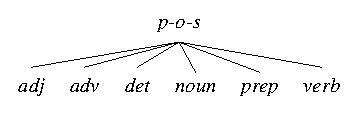
\includegraphics{types-pos.eps}}}
\end{itemize}
}


%\iftoggle{loesungen}{
\frame{
\frametitle{Merkmalbeschreibungen vom Typ {\it person\/}}

\begin{itemize}
\item Unsere Beispielbeschreibung beschreibt Objekte vom Typ {\it person\/}.
\scalebox{0.8}{\ms[\blau{person}]{
vorname    & max\\
nachname   & meier\\
geburtstag & 10.10.1985\\
geschlecht & männlich\\
vater      & \ldots\\
mutter     & \ldots\\
kinder     & \liste{ \ldots, \ldots }\\   
}
}

\item Eigenschaften wie {\sc Betriebsspannung} sind für solche Objekte nicht relevant!


\item Typ sagt, welche Merkmale zu einem solchen Objekt gehören.

\item Wissen, dass jeder Mensch einen Geburtstag hat,\\
auch wenn wir diesen nicht kennen.
\end{itemize}
}
%}%\end{loesungen}

\subsection{Strukturteilung}

\handoutframe{
\frametitle{Strukturteilung}

Werte von A1 und A2 sind token-identisch:

\ms{A1 & \ibox{1} \mbox{\rm [{\sc A3}  {\it W3}]} \\
    A2 & \ibox{1} \\
   }

Die Identität der Werte wird durch Boxen verdeutlicht.

Boxen kann man als Variablen auf"|fassen.

%%\bigskip

%% \pause
%% unser Kongruenzbeispiel

%% \begin{tabular}[t]{@{}l@{ }l}
%% S  & $\to$ NP(Agr,nom), NP(Agr2,dat), NP(Agr3,acc), V(Agr)\\
%% \end{tabular}

%% mit Merkmalsbeschreibungen:
%% \begin{tabular}[t]{@{}l@{ }l}
%% [{\sc cat} S]  $\to$ & [{\sc cat} NP, {\sc agr} \ibox{1}, {\sc cas} {\it nom}], \\
%%                      & [{\sc cat} NP, {\sc cas} {\it dat\/}], \\
%%                      & [{\sc cat} NP, {\sc cas} {\it acc}], [{\sc cat} V, {\sc agr} \ibox{1}]\\
%% \end{tabular}

}

 
%\iftoggle{loesungen}{
\frame{

\small
\frametitle{\normalsize Unser Beispiel mit Kindern (I)}

\begin{itemize}
\item Beschreiben wir ein Kind oder zwei Kinder von Peter und Anna?
\scalebox{0.7}{\ms[person]{
vorname    & max\\
nachname   & meier\\
geburtstag & 10.10.1985\\
vater      & \ms[person]{
              vorname  & peter\\
              nachname & meier\\
              kinder   & \liste{ \blau{\ms[person]{
                                 vorname & klaus\\
                                 }, \ldots }}\\
             }\\
mutter     & \ms[person]{
              vorname  & anna\\
              nachname & meier\\
              kinder   & \liste{ \blau{\ms[person]{
                                 vorname & klaus\\
                                 }, \ldots }}\\
             }\\
}
}

\item Wir wissen es nicht!


\item Es können zwei Kinder aus früheren Verbindungen sein.
\end{itemize}
}


\frame{

\small
\frametitle{\normalsize Unser Beispiel mit Kindern (II)}

\begin{itemize}
\item Beschreiben wir ein Kind oder zwei Kinder von Peter und Anna?
\scalebox{0.7}{\ms[person]{
vorname    & max\\
nachname   & meier\\
geburtstag & 10.10.1985\\
vater      & \ms[person]{
              vorname  & peter\\
              nachname & meier\\
              kinder   & \liste{ \ibox{1} \ms[person]{
                                 vorname & klaus\\
                                 }, \ldots }\\
             }\\
mutter     & \ms[person]{
              vorname  & anna\\
              nachname & meier\\
              kinder   & \liste{ \ibox{1}, \ldots }\\
             }\\
}}

\item Klaus ist ein Kind, das beide gemeinsam haben.

\item Was ist mit Max?
\end{itemize}
}

\subsection{Zyklische Beschreibungen}

\frame{
\frametitle{Unser Beispiel mit Kindern -- Zyklische Beschreibungen}


\begin{itemize}
\item \ibox{2} steht vor der gesamten Beschreibung und kommt auch in ihr vor.
\scalebox{0.8}{\ibox{2} \ms[person]{
vorname    & max\\
nachname   & meier\\
geburtstag & 10.10.1985\\
vater      & \ms[person]{
              vorname  & peter\\
              nachname & meier\\
              kinder   & \liste{ \ibox{1} \ms[person]{
                                 vorname & klaus\\
                                 }, \ibox{2} }\\
             }\\
mutter     & \ms[person]{
              vorname  & anna\\
              nachname & meier\\
              kinder   & \liste{ \ibox{1}, \ibox{2} }\\
             }\\
}
}
\end{itemize}

}


%}%\end{loesungen}

\subsection{Unifikation}

\frame{
\frametitle{Unifikation}

\begin{itemize}
\item Grammatikregeln \& Lexikoneinträge werden durch Merkmalbeschreibungen beschrieben. 
\item Grammatikregeln enthalten Beschreibungen möglicher Töchter,\\
      aber nicht die vollständige Information über die Tochter.
\item Im konkreten Fall muss eine Phrase mit den Anforderungen an die Tochter\\
      kompatibel sein, um in einer Struktur als Tochter vorkommen zu dürfen.
\item Bezeichnung für diese spezielle Art der Kompatibilität: \blaubf{Unifizierbarkeit}
\item Wenn man zwei Strukturen unifiziert, bekommt man eine Struktur,\\
      die die Information aus den beiden unifizierten Strukturen enthält,\\
      aber keine zusätzliche Information.
\end{itemize}


}

\frame{
\frametitle{Beispiel: Detektivbüro}

\begin{itemize}
\item Wir suchen nach einer blonden, weiblichen Person namens Meier.

\item Die Merkmalbeschreibung wäre:\\
\medskip
\ms[person]{
nachname   & meier\\
geschlecht & weiblich\\
haarfarbe  & blond\\
}

\item Wenn wir als Antwort folgende Beschreibung bekommen,\\
      wechseln wir das Büro.\\
\medskip
\ms[person]{
nachname   & meier\\
geschlecht & männlich\\
haarfarbe  & rot\\
}

\end{itemize}

}

\frame{
\frametitle{Beispiel: Detektivbüro}
\smallframe

\begin{itemize}
\item Wir suchen nach einer blonden, weiblichen Person namens Meier.

\scalebox{0.9}{\ms[person]{
nachname   & meier\\
geschlecht & weiblich\\
haarfarbe  & blond\\
}}

ein mögliches Ergebnis für eine Anfrage:

\scalebox{0.9}{\ms[person]{
vorname    & katharina\\
nachname   & meier\\
geschlecht & weiblich\\
geburtstag & 15.10.1965\\
haarfarbe  & blond\\
}}

\item Katharina Meier kann weitere Eigenschaften haben,\\ die der Detektiv nicht kennt.

Wichtig ist nur, dass die, die er kennt, zur Anfrage passen.

\end{itemize}

}

\frame{
\frametitle{Beispiel: Detektivbüro}

\begin{tabular}{@{}l@{\hspace{2em}}l@{}}
Die Unifikation der Anfrage & mit der Information des Detektivs\\
\scalebox{0.85}{\ms[person]{
nachname   & meier\\
geschlecht & weiblich\\
haarfarbe  & blond\\
}} & \scalebox{0.85}{\ms[person]{
vorname    & katharina\\
nachname   & meier\\
geschlecht & weiblich\\
geburtstag & 15.10.1965\\
haarfarbe  & blond\\
}}\\
\multicolumn{2}{@{}l@{}}{%
\alt<beamer>{ist \visible<2>{und \rot{nicht} etwa:}}{ist nicht folgendes, da keine Information über Kinder vorliegt:}}\\
\scalebox{0.85}{\ms[person]{
vorname    & katharina\\
nachname   & meier\\
geschlecht & weiblich\\
geburtstag & 15.10.1965\\
haarfarbe  & blond\\
\visible<2>{\rot{kinder}} & \visible<2>{\rot{\liste{}}}\\
}} & \begin{tabular}{@{}l@{}}
     \visible<2>{Der Detektiv darf sich nichts ausdenken!}\\
     \visible<2>{Er riskiert sonst seinen Job!}\\
     \end{tabular}
\end{tabular}

}

\subsection{Phänomene, Modelle und formale Theorien}

\frame{
\frametitle{Phänomene, Modelle und formale Theorien}

\hfill
\begin{pspicture}(0,0)(10.4,5)
%\psgrid
\rput[Bl](0,0){%
\begin{tabular}[b]{@{}ccc@{}}
Phänomen && Modell\\
\rnode{phen}{\fbox{\begin{tabular}{c}
Linguistische\\
Objekte\\
\end{tabular}}}&&\rnode{modell}{\fbox{\begin{tabular}{c}
Merkmal-\\
strukturen\\
\end{tabular}}}\\[10ex]
&\rnode{theorie}{\fbox{\begin{tabular}{c}
Merkmal-\\
beschreibungen\\
\end{tabular}}}\\
&Formale Theorie\\
\end{tabular}}
%\anodeconnect[l]{modell}[r]{phen}%
\ncline{->}{modell}{phen}\nbput{modelliert}
%\ncdiag[angleA=180,angleB=45]{->}{modell}{theorie}
\psline{<-}(6.0,1.6)(6.6,2.4)
\rput[Bl](6.6,2){wird von Theorie lizenziert} % früher Erfüllung, jetzt FR Änderung
\psline{->}(5.6,1.6)(6.2,2.4)
\rput[Bl](4.5,2.4){legt fest}
%\nccurve{<-}{modell}{theorie}\nbput{legt fest}
\ncline{->}{theorie}{phen}\naput{sagt vorher}%
%\aanodeconnect[b]{modell}[tr]{theorie}%
%\anodeconnect[tl]{theorie}[b]{phen}%
\end{pspicture}\hfill\hfill\mbox{}
}



\subsection{Hausaufgaben}

\frame[shrink=15]{
\frametitle{Hausaufgaben}

\begin{enumerate}
\item Überlegen Sie, wie man Musikinstrumente mittels Merkmalstrukturen beschreiben könnte.
\item In diesem Kapitel wurden Listen eingeführt. Dies sieht wie eine Erweiterung des Formalismus
      aus. Dem ist aber nicht so, denn man kann die Listennotation in eine Notation überführen,
      die nur mit Merkmal"=Wert"=Paaren auskommt. Überlegen Sie wie das geht.
\item Im folgenden Kapitel wird die Relation \emph{append}\is{Relation!\emph{append}} eine Rolle spielen, die dazu dient,
      zwei Listen zu einer dritten zu verknüpfen. Relationale Beschränkungen stellen eine Erweiterung
      des Formalismus dar. Man kann beliebige Werte von Merkmalen zu anderen Werten in Beziehung setzen.
      Es stellt sich die Frage, ob man solch mächtige Beschreibungsmittel in einer linguistischen
      Theorie braucht und wenn man sie zuläßt, was für eine Komplexität man ihnen zubilligt. Eine
      Theorie, die ohne relationale Beschränkungen auskommt, ist einer anderen vorzuziehen.

      Für die Verkettung von Listen gibt es eine direkte Umsetzung in Merkmalstrukturen ohne
      relationale Beschränkungen. Finden Sie diese. Geben Sie Ihre Quellen an und dokumentieren Sie,
      wie Sie bei der Suche nach der Lösung vorgegangen sind.
\end{enumerate}

}

% \begin{comment}
% \frame{

% \frametitle{Strukturteilung}

% \eal
% \ex[]{
% Hans schläft.
% }
% \ex[*]{
% Hans schläfst.
% }
% \zl

% \begin{mydefinition}
% Zwei Merkmale innerhalb einer Merkmalstruktur \blau{teilen sich eine
% gemeinsame Struktur}, wenn beide denselben Wert haben.
% Diese Gleichheit bleibt auch bei Veränderungen an der
% Merkmalstruktur bestehen.
% Der gemeinsame Wert wird nur einmal in die Merkmalstruktur
% eingetragen, die Übereinstimmung wird durch einen Index
% festgelegt.
% \end{mydefinition}

% andere Bezeichnungen: Koreferenz, {\it reentrancy\/}

% }

% \frame{
% \frametitle{Strukturteilung}

% A1 und A2 sind token-identisch:

% \(
% \ms{A1 & \ibox{1} \ms{ A3 & W3 \\
%                      } \\
%     A2 & \ibox{1} \\
%    }
% \)

% A1 und A2 sind gleich:

% \(
% \ms{A1 & \ms{ A3 & W3 \\
%                      } \\
%     A2 & \ms{ A3 & W3 \\
%             }  \\
%    }
% \)

% Unterschied bei Strukturmanipulation
% }
% \frame{
% \frametitle{Subjekt-Verb-Kongruenz mit Strukturteilung}


% \eal
% \ex[]{
% Hans schläft.
% }
% \ex[*]{
% Hans schläfst.
% }
% \zl

% \(
% \label{hans1}
% \ms{ subj & \ms{ phon & hans \\
%                  agr  & \ibox{1} \ms{ num & sg \\
%                                       per & 3 \\
%                                     } \\
%                } \\
%      pred & \ms{ phon & schläft \\
%                  agr  & \ibox{1} \\
%                } \\
%     }
% \)

% }

% \frame{
% \frametitle{Subjekt-Verb-Kongruenz in Graphendarstellung}

% \begin{center}
% \setlength{\unitlength}{0.01in}%
% \begin{picture}(280,266)(70,560)
% \put(238,795){\circle{20}}  % hans
% \put(238,585){\circle{20}}  % schläft
% \put(238,690){\circle{20}}  % agr
% \put(138,745){\circle{20}}  % subj
% \put(138,635){\circle{20}}  % pred
% \put(338,740){\circle{20}}  % 3
% \put(338,640){\circle{20}}  % sg
% \put( 43,690){\circle{20}}
% \put(148,750){\vector( 2, 1){ 80}}
% \put(148,740){\vector( 2,-1){ 82}}
% \put(148,640){\vector( 2, 1){ 82}}
% \put(148,630){\vector( 2,-1){ 80}}
% \put(248,695){\vector( 2, 1){ 80}}
% \put(248,685){\vector( 2,-1){ 80}}
% \put( 48,700){\vector( 2, 1){ 80}}
% \put( 48,680){\vector( 2,-1){ 80}}
% \put( 13,690){\vector( 1, 0){ 20}}
% \put( 40,725){\makebox(0,0)[lb]{{\sc subj}}}
% \put( 40,640){\makebox(0,0)[lb]{{\sc pred}}}
% \put(150,780){\makebox(0,0)[lb]{{\sc phon}}}
% \put(150,590){\makebox(0,0)[lb]{{\sc phon}}}
% \put(150,710){\makebox(0,0)[lb]{{\sc agr}}}
% \put(150,665){\makebox(0,0)[lb]{{\sc agr}}}
% \put(250,725){\makebox(0,0)[lb]{{\sc per}}}
% \put(250,640){\makebox(0,0)[lb]{{\sc num}}}
% \put(360,635){\makebox(0,0)[lb]{{\it sg}}}
% \put(360,735){\makebox(0,0)[lb]{{\it 3}}}
% \put(260,790){\makebox(0,0)[lb]{{\it hans}}}
% \put(260,580){\makebox(0,0)[lb]{{\it schläft}}}
% \end{picture}
% \end{center}
% }

% \frame{

% \frametitle{Subsumption}

% 

% \begin{mydefinition}
% Eine Merkmalstruktur M1 \blau{subsumiert} eine Merkmalstruktur
% M2 (M1 $\succeq$  M2), wenn folgendes gilt: 
% \begin{itemize}
% \item Jeder vollständige Pfad von M1 ist als vollständiger Pfad 
%       in M2 enthalten und hat dort denselben Wert wie in M1.
% \item Jedes Paar von Pfaden in M1, das denselben Wert hat 
% 	({\it structure sharing}\/), mu"s auch in M2 denselben Wert haben.
% \end{itemize}
% \end{mydefinition}

% 

% }

% \frame{
% 
% {\footnotesize
% \frametitle{Beispiele}

% M1 $\succeq$  M2 $\succeq$  M7 $\succeq$  M8 $\succeq$  M9
                                    
% M1 $\succeq$  M4 $\succeq$  M6 $\succeq$  M7 $\succeq$  M8 $\succeq$  M9
                                    
% M1 $\succeq$  M3
                                    
% M1 $\succeq$  M4 $\succeq$  M5

% \begin{tabular}{p{3.0cm}p{3.0cm}p{3.0cm}}
% M1:       $[~]$            \\ \\
% M2:       $\ms{ cat & np \\ }$    & M3:       $\ms{ cat & vp \\} $   & M4:       $\ms{ agr$|$per & 3 \\ } $ \\
% \end{tabular}

% \begin{tabular}{p{3.0cm}p{4.0cm}p{3.0cm}}
% M5:       $\ms{ agr & \ms{ num & pl \\
%                            per & 3  \\
%                          } \\ }$  &           
% M6:       $\ms{ agr & \ms{ num & sg\\
%                            per & 3  \\
%                          } \\ }$ \\
% \end{tabular}

% \begin{tabular}{p{3.0cm}p{3.0cm}p{4.0cm}}
% M7:       $\ms{ cat & np \\
%                 agr & \ms{ num & sg\\ 
%                            per & 3  \\
%                          } \\ }$ &
% %
% M8:       $\ms{ cat & np \\
%                 agr & \ms{ num & sg\\ 
%                            per & 3  \\
%                          } \\
%                 subj & \ms{  num & sg\\ 
%                            per & 3  \\
%                          } \\
%                }$ &
% %
% M9:        $\ms{ cat & np \\
%                 agr & \ibox{1} \ms{ num & sg\\ 
%                            per & 3  \\
%                          } \\
%                 subj & \ibox{1} \\ 
%                }$ \\
% \end{tabular}
% }
% }

% \frame{

% \frametitle{Unifikation}
% 

% \is{$\wedge$}
% \begin{mydefinition}
% M1, M2 und M3 seien Merkmalstrukturen. M3 ist genau dann
% \blau{Unifikation} von M1 und M2 (M3 = M1 $\wedge$ M2), wenn 
% \begin{itemize}
% \item M3 von M1 und M2 subsumiert wird und
% \item M3 alle anderen Merkmalstrukturen M subsumiert, die
%    ebenfalls von M1 und M2 subsumiert werden.
% \end{itemize}
% \end{mydefinition}
% 

% }
% \frame{
% \frametitle{Beispiele}
% \(
% \ms{ cat & np \\ } \wedge \ms{cat & np\\ } = \ms{ cat & np \\ }
% \)
% \( 
% \ms{ cat & np \\ } \wedge \ms{ agr & \ms{ per & 3 \\
%                                           num & sg \\
%                                         } \\
%                              } = \ms{ cat & np \\
%                                       agr & \ms{ per & 3 \\
%                                                  num & sg \\
%                                                } \\
%                                     } \\
% \)
% \(
% \ms{ cat & np \\ } \wedge \ms{ agr & \ms{ per & 3 \\
%                                           num & sg \\
%                                         } \\
%                              } \neq \ms{ cat & np \\
%                                       agr & \ms{ per & 3 \\
%                                                  num & sg \\
%                                                } \\
%                                       subj & \ms{  num & sg \\ } \\
%                                     } \\
% \)

% }

% \frame{
% \frametitle{Unifikation und Strukturteilung}
% 


% \(
% \ms{ agr & \ibox{1} \ms{ num & sg \\ } \\
%      subj & \ibox{1} \\
%    } \wedge
% \ms{ subj & \ms{ per & 3 \\ } \\
%    } = 
% \ms{ agr & \ibox{1} \ms{ num & sg \\ 
%                          per & 3 \\
%                        } \\
%      subj & \ibox{1} \\
%    } 
% \)
% \(
% \ms{ agr & \ms{ num & sg \\ } \\
%      subj & \ms{ num & sg \\ }  \\
%    } \wedge
% \ms{ subj & \ms{ per & 3 \\ } \\
%    }  = 
% \ms{ agr & \ms{ num & sg \\ 
%               } \\
%      subj & \ms{ num & sg \\ 
%                  per & 3 \\
%                 }  \\
%    } 
% \)
% 

% }
% \frame{

% \frametitle{Negation, Disjunktion und Implikation}

% Unifikation entspricht Konjunktion

% andere Verknüpfungen: Negation, Disjunktion und Implikation

% atomare Werte:

% \begin{table}[H]
% \begin{tabular}{@{}lr@{~$\vee$~}l}
% Person  & 1  & 3  \\
% Numerus & sg & pl \\
% \end{tabular}
% \end{table}

% komplex

% \(
% \label{mdie}
% M_{die} = 
% \ms{ cas & nom $\vee$ acc \\
%      agr & \ms{ gen & fem \\
%                 num & sg \\
%               } $\vee$
%            \ms{ num & pl \\ } \\
%    }
% \)

% }
% \frame{
% \frametitle{Unifikation von Merkmalstrukturen mit Disjunktionen}

% Unifikation: Kreuzprodukt aller Disjunkte

% \(
% M_{die} = 
% \ms{ cas & nom $\vee$ acc \\
%      agr & \ms{ gen & fem \\
%                 num & sg \\
%               } $\vee$
%            \ms{ num & pl \\ } \\
%    }
% \)
% \(
% M_{Menschen} =
% \ms{ cas & gen $\vee$ dat $\vee$ acc \\
%       agr & \ms{ gen & mas \\ } \\
%     } \vee
%  \ms{ cas & nom \\
%       agr & \ms{ gen & mas \\
%                  num & pl \\
%                } \\
%     }
% \)
% %
% \(
% M_{die}~\wedge   M_{Menschen} =
% \ms{ cas & nom $\vee$ acc \\
%       agr & \ms{ gen & mas \\
%                  num & pl \\
%                } \\
%     }
% \)

% }

% \frame{
% \frametitle{Implikation}

% \is{Implikation}
% \is{$\Rightarrow$}
% %Wäh\-rend wir die Disjunktion auf allen Ebenen der Merkmalstrukturen
% %betrachtet haben, ist die Implikation A $\Rightarrow$  B nur auf der
% %Ebene vollständiger Merkmalstrukturen sinnvoll.
% Mit der Implikation A $\Rightarrow$ B werden bestimmte Prinzipien ausgedrückt,
% die für Merkmalstrukturen innerhalb linguistischer Theorien
% gelten. Ihre Bedeutung wird bei der Behandlung der Prinzipien der HPSG klarer werden.

% Die Implikation zweier Merkmalstrukturen A und B (A $\Rightarrow$  B)
% ist die am wenigsten informative Merkmalstruktur, deren
% Unifikation mit A von B subsumiert wird.

% Daraus folgt:
% Wenn ein linguistisches Objekt X sowohl von einer Merkmalstruktur C 
% als auch von A $\Rightarrow$  B beschrieben wird und C
% von A subsumiert wird, dann ist jede Merkmalstruktur C',
% C' = C $\wedge$  B, auch eine Beschreibung für X.

% \subsection*{Negation}

% \is{Negation}
% Die Negation von Merkmalstrukturen kann anstelle einer Disjunktion 
% eingesetzt werden. Die Negation atomarer Merkmalstrukturen ist stets
% durch eine Disjunktion ersetzbar, wenn man voraussetzt, 
% da"s bekannt ist, welche Werte ein Merkmal annehmen kann.

% (\mex{1}) zeigt ein Beispiel.
% %
% \eq{
% \ms{ num & pl\\} \vee 
% \ms{ per & 1 \\
%      num & sg \\
%     } \vee
% \ms{ per & 2 \\
%      num & sg \\
%     } =
% \neg \ms{ per & 3 \\
%           num & sg \\
%          } \\
% }
% $\neg$ A entspricht au"serdem der Implikation A $\Rightarrow$ $\bot$.

% \frame{
% \frametitle{Listen}
% 

% \begin{mydefinition} 
% Eine Liste A = \liste{ A$_1$, \ldots, A$_n$} \blau{subsumiert}
% eine Liste B = \liste{ B$_1$, \ldots, B$_n$ } (A $\succeq$ B) gdw.
% jedes $A_i$ das dazugehörige $B_i$ subsumiert ($A_i \succeq B_i$, 
% i = 1, \ldots, n).
% \end{mydefinition}
% 
% \begin{mydefinition}
% Seien A = \liste{ A$_1$, \ldots, A$_n$}, B = \liste{ B$_1$, \ldots, B$_n$ } und 
% C = \liste{ C$_1$, \ldots, C$_n$} Listen von Merkmalstrukturen.
% C ist die \blau{Unifikation} von A und B (C = A $\wedge$ B) gdw.
% für jedes $C_i$ gilt $C_i = A_i \wedge B_i$.
% \end{mydefinition}
% 
% \liste{} steht für die leere Liste, \dash, für eine Liste ohne Elemente
% 
% Listen kann man auch als Merkmal-Wert-Paare aufschreiben $\to$ Klammerschreibweise
% ist nur Abkürzung
% 
% }
% \frame{
% \frametitle{Funktionen und Relationen}
% 


% \begin{tabbing}
% $append($ \= \liste{X$_1$,X$_2$, \ldots, X$_n$},\liste{Y$_1$,Y$_2$, \ldots, Y$_m$})~= \\[1mm]
%           \> \liste{X$_1$,X$_2$, \ldots, X$_n$,Y$_1$,Y$_2$, \ldots, Y$_m$}
% \end{tabbing}

% \(
% \ms{
% A & \ibox{1} $\oplus$ \ibox{2} \\
% B & \ibox{1}\\
% C & \ibox{2}\\
% }
% \)
% 

% }

% \frame{

% \frametitle{Getypte Merkmalstrukturen}
% \label{tms}
% 


% keinerlei Einschränkungen für die Wahl von Merkmalen und ihren Werten

% \(
% \ms{ agr & \ms{ per & 3 \\
%                       num & sg \\
%                     }\\
%           }
% \)

% \(
%        \ms{ farbe & blau \\ }
% \)

% kompatibel, obwohl total verschiedene Objekte beschrieben werden

% 
% Negation und Disjunktion

% $\neg$[{\sc num} {\it pl\/}] $\stackrel{?}{=}$ [{\sc num} {\it sg\/}] $\vee$ [{\sc num} {\it 17\/}] $\vee$
% [{\sc farbe} {\it blau\/}]

% Informationen unbekannt oder irrelevant oder unpassend
% 

% }

% \frame{
% 
% \footnotesize

% \frametitle{\small Typen und Appropriateness}
% 

% Merkmale werden in der Definition eines Typs eingeführt

% Beispiel:

% \(
% \ms[constr]{ phon & hans \\
%             agr  & \ms[agr]{ per & 3 \\
%                            num & sg \\
%                          }\\
%                  }
% \hspace{2.5cm}
% \ms[constr]{ phon & string \\
%             agr  & agr\\
%           }\hspace{1cm}
% \ms[agr]{ per & per \\
%           num & num \\
%         }
% \)

% Typdefinition: \begin{tabular}[t]{@{}l}
%                Merkmalstrukturen vom Typ {\it constr\/} haben immer die Merkmale {\sc phon} und {\sc agr}\\
%                Merkmalstrukturen vom Typ {\it agr\/} haben immer die Merkmale {\sc per} und {\sc num}\\
%                \end{tabular}


% komplexe Typen:

% \(
% \ms[3rd-sg-constr]{ phon & string \\
%             agr  & \ms[agr]{ per & 3 \\
%                              num & sg \\
%                            }\\
%                    }
% \)

% 

% }

% \frame{
% \frametitle{Getypte Merkmalstruktur}
% 
% \(
% \label{hans2}
% \ms[satz]{ 
%      subj & \ms[constr]{ 
%               phon & \ms[hans]{}  \\
%               agr  & \ibox{1}\ms[agr]
%                                  { num & \ms[sg~]{} \\
%                                    per & \ms[3~]{} \\
%                                  } \\
%                } \\
%      pred & \ms[constr]{ 
%                  phon & \ms[schläft]{} \\
%                  agr  & \ibox{1} \\
%                } \\
%     }
% \)
% 

% }

% \frame{
% \frametitle{Getypte Merkmalstruktur in Graphendarstellung}

% \begin{center}
% \setlength{\unitlength}{0.01in}%
% \begin{picture}(280,266)(70,560)
% \put(238,795){\circle{20}}  % hans
% \put(238,585){\circle{20}}  % schläft
% \put(238,690){\circle{20}}  % agr
% \put(138,745){\circle{20}}  % subj
% \put(138,635){\circle{20}}  % pred
% \put(338,740){\circle{20}}  % 3
% \put(338,640){\circle{20}}  % sg
% \put( 43,690){\circle{20}}
% \put(148,750){\vector( 2, 1){ 80}}
% \put(148,740){\vector( 2,-1){ 82}}
% \put(148,640){\vector( 2, 1){ 82}}
% \put(148,630){\vector( 2,-1){ 80}}
% \put(248,695){\vector( 2, 1){ 80}}   
% \put(248,685){\vector( 2,-1){ 80}}
% \put( 48,700){\vector( 2, 1){ 80}}
% \put( 48,680){\vector( 2,-1){ 80}}
% \put( 13,690){\vector( 1, 0){ 20}}
% \put( 40,725){\makebox(0,0)[lb]{{\sc subj}}}
% \put( 40,640){\makebox(0,0)[lb]{{\sc pred}}}
% \put(150,780){\makebox(0,0)[lb]{{\sc phon}}}
% \put(150,590){\makebox(0,0)[lb]{{\sc phon}}}
% \put(150,710){\makebox(0,0)[lb]{{\sc agr}}}
% \put(150,665){\makebox(0,0)[lb]{{\sc agr}}}
% \put(250,725){\makebox(0,0)[lb]{{\sc per}}}
% \put(250,640){\makebox(0,0)[lb]{{\sc num}}}
% \put( 65,685){\makebox(0,0)[lb]{{\it satz}}}
% \put(165,740){\makebox(0,0)[lb]{{\it constr}}}
% \put(165,630){\makebox(0,0)[lb]{{\it constr}}}
% \put(265,685){\makebox(0,0)[lb]{{\it agr}}}
% \put(360,635){\makebox(0,0)[lb]{{\it sg}}}
% \put(360,735){\makebox(0,0)[lb]{{\it 3}}}
% \put(260,790){\makebox(0,0)[lb]{{\it hans}}}
% \put(260,580){\makebox(0,0)[lb]{{\it schläft}}}
% \end{picture}
% \end{center}

% }

% \frame{
% 
% {\small
% \frametitle{Subsumption und Unifikation mit Typen}

% Die Definitionen sind analog zu denen der Merkmalstrukturen:
% %
% \is{Subsumption!Definition!Typen}
% \is{$\succeq$}
% \begin{mydefinition}
% Ein Typ t1 \blau{subsumiert} einen Typ t2 (t1 $\succeq$ t2), wenn gilt:
% \begin{itemize}
% \item Wenn t1 und t2 selbst keine Struktur haben, dann mu"s t1 mindestens so allgemein
%       wie t2 sein.
% \item Wenn t1 und t2 eine Struktur haben, dann mu"s t1 mindestens so allgemein 
%       wie t2 sein und es mu"s gelten:
%       Jedes Merkmal {\sc attr}, das in Merkmalstrukturen vom Typ t1 vorkommt, mu"s auch in 
%       Merkmalstrukturen vom Typ t2 vorkommen,
%       und für die ATTR zugeordneten Typen t1$_{ATTR}$ und t2$_{ATTR}$ gilt:
%       t1$_{ATTR}$ $\succeq$ t2$_{ATTR}$.
% \end{itemize}
% \end{mydefinition}
% %
% Man sagt, {\it t1\/} ist \blau{Supertyp} von {\it t2\/} bzw.\ {\it t2\/} ist \blau{Subtyp} von {\it t1\/}.

% \is{Unifikation!Definition!Typen}
% \begin{mydefinition}
% t1, t2 und t3 seien Typen. t3 ist dann die \blau{Unifikation} von t1 und t2, wenn 
% \begin{itemize}
% \item t3 von t1 und t2 subsumiert wird und
% \item t3 alle anderen Typen t subsumiert, die ebenfalls von t1 und t2 subsumiert werden.
% \end{itemize}
% \end{mydefinition}
% }
% }

% \frame{
% \frametitle{Ein Beispiel}

% 

% \(
% A = \ms[aa]{
% a1 & a\\
% a2 & \ms[b]{ a21 & c\\
%            }\\
% }
% \hspace{2cm}
% B = \ms[bb]{
% a1 & a\\
% a2 & \ms[d]{ a21 & c\\
%            }\\
% a3 & e\\
% }
% \)

% A $\succeq$ B, wenn aa $\succeq$ bb und b $\succeq$ d

% 
% }

% \frame{
% \frametitle{Atomare und komplexe Typen in Vererbungshierarchien}


% 

% atomare:
% \begin{figure}[htbp]
% \epsfxsize=0.1\textwidth
% \centerline{\mbox{\epsffile{type-per.eps}}}
% \end{figure}

% genauso komplexe Typen

% 
% }

% \frame{
% \frametitle{Ein nichtlinguistisches Beispiel für Mehrfachvererbung}

% 

% \begin{figure}[htbp]
% \epsfxsize=0.6\textwidth
% \centerline{\mbox{\epsffile{type-elektr-geraet.eps}}}
% \end{figure}

% 

% }

% \frame{

% \frametitle{Negierte Subtypen} 

% 

% \begin{figure}[htp]
% \begin{center}
% \setlength{\unitlength}{0.012500in}%
% \begin{picture}(85,89)(120,680)
% \put(165,755){\line(-5,-2){ 39.655}}
% \put(165,755){\line( 0,-1){ 15}}
% \put(165,755){\line( 5,-2){ 39.655}}
% \put(125,715){\line( 0,-1){ 15}}
% \put(165,715){\line( 0,-1){ 15}}
% \put(205,715){\line( 0,-1){ 15}}
% \put(205,715){\line(-5,-1){ 79.808}}
% \put(165,715){\line( 5,-2){ 39.655}}
% \put(125,715){\line( 5,-2){ 39.655}}
% \put(160,760){\makebox(0,0)[lb]{{\it per }}}
% \put(120,720){\makebox(0,0)[lb]{{\it not1}}}
% \put(160,720){\makebox(0,0)[lb]{{\it not2}}}
% \put(200,720){\makebox(0,0)[lb]{{\it not3}}}
% \put(125,680){\makebox(0,0)[lb]{{\it 2}}}
% \put(165,680){\makebox(0,0)[lb]{{\it 3}}}
% \put(205,680){\makebox(0,0)[lb]{{\it 1}}}
% \end{picture}
% \end{center}
% \end{figure}

% 
% }
% \end{comment}

% \frame{
% \frametitle{Types}

% \begin{itemize}
% \item type hierarchies for lexical types and phrasal types
% \item linguistic generalizations are captured in the type hierarchies
% \item multiple inheritance
% \end{itemize}

% \bigskip
% \begin{itemize}
% \item \begin{itemize}
%       \item lexical types:\\
%       \citet{Flickinger87}, \citet{AW98a}, \citet{Koenig99a}
%       \item phrasal types:\\
%       \citet{Sag97a}
%       \end{itemize}
% \end{itemize}
% }


